\documentclass[12pt,letterpaper]{article}

%\pagenumbering{gobble} % arabic, roman, Roman, alph, Alph
\pagenumbering{arabic} % arabic, roman, Roman, alph, Alph
%\setcounter{page}{0} % sets the initial page

\oddsidemargin = -0.25 in
\evensidemargin = -0.25 in
\topmargin = -0.5 in
\headheight = 0 in
%\headsep = 0.5 in
%\topskip = 0 in
\textheight = 9 in
\textwidth = 6.75 in
\footskip = 0.5 in

\usepackage{notes}
\usepackage{graphicx}
\usepackage{tcolorbox}

%\voffset = -0.5 in
%\hoffset = -0.5 in

\parskip 10 pt

\font\sf = cmss10

\setlength\parindent{0pt}




\begin{document}

\thispagestyle{empty}

\baselineskip = 15 pt % between lines

% sanscrif \tt

MATH 180 NOTES \hfill Section 6.1: Areas Between Curves

\hrulefill

Goal: Find the area between two curves of $y = f(x)$ and $y = g(x)$.

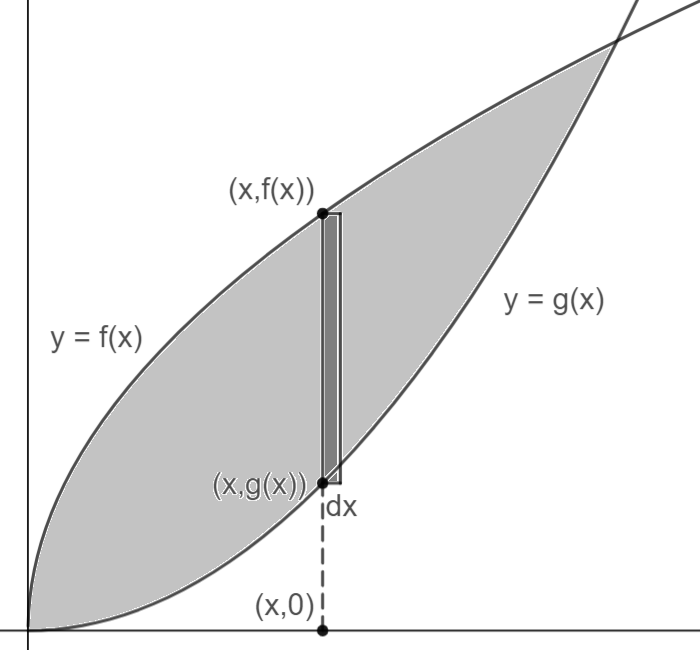
\includegraphics[scale=0.7]{math180_sec6_1_img1r.png}




\end{document}
